%==============================
\subsection{Task Decomposition}\label{subsubsec:task-decompose}
Since the team-wise task in this work is given as a compact temporal task formula,
a prerequisite for optimal task assignment later is to decompose this task into suitable subtasks.
Moreover, different from simple reachability task,
temporal tasks can impose strict constraints on the ordering of sub-tasks.
For instance, the task~$\Diamond (\omega_1 \land \Diamond (\omega_2 \land \Diamond\omega_3)) $
specifies that $\omega_1,\omega_2,\omega_3$ should be satisfied in sequence,
while~$\Diamond\omega_1\land\Diamond\omega_2\land\Diamond\omega_3$ does not impose any ordering constraint.
Thus, it is essential for the overall correctness to abstract such ordering constraints among the subtasks.
This part describes how the subtasks and their partial orderings are abstracted from the pruned automaton~$\mathcal{B}_{\varphi}^{-}$.

\begin{definition}[Decomposition and Subtasks] \label{def:subtasks}
Consider an accepting run $\rho=q_0q_1\cdots q_L$ of~$\mathcal{B}_{\varphi}^{-}$,
where $q_0\in Q_0$ and $q_L\in Q_F$.
One \emph{possible} decomposition of $\varphi$ into subtasks is defined
as a set of 3-tuples:
\begin{equation}\label{eq:subtask}
\Omega_{\varphi} = \left\{(\ell,\, \sigma_\ell,\, \sigma^{s}_\ell),\, \forall \ell=1,\cdots,L\right\},
\end{equation}
where $\ell$ is the index of subtask~$\sigma_\ell$,
and $\sigma_\ell\subseteq \Sigma$ satisfies two conditions:
(i) $q_{\ell+1} \in \delta(q_{\ell-1},\,\sigma_\ell)$;
and (ii) $q_{\ell+1} \notin \delta(q_\ell,\,\sigma^-_\ell)$, where~$\sigma^-_\ell =  \sigma_\ell \backslash \{s\}$, $\forall s\in \sigma_\ell$,
and $\sigma^{s}_\ell\subseteq \Sigma$ also satisfies two conditions:
(i) $q_{\ell-1} \in \delta(q_{\ell-1},\,\sigma^{s}_\ell)$;
and (ii) $q_{\ell-1} \notin \delta(q_{\ell-1},\,\sigma^{s-}_\ell)$, where~$\sigma^{s-}_\ell =  \sigma^{s-}_\ell \backslash \{s\}$, $\forall s\in \sigma^{s-}_\ell$.
\hfill $\blacksquare$
\end{definition}

\begin{example}
	\label{example:subtask}
        {As shown in Fig.~\ref{fig:example_decomposable},
          the subtasks associated with~$q_1q_2\\q_4q_5$ are given
          by~$\Omega=\{(1,\texttt{sweep}_{p_{21}} ,\lnot p_{24}),
(1,\texttt{mow}_{p_{21}} ,\lnot p_{24}),\\
(1,\texttt{scan}_{p_{21}}\land\lnot \texttt{mow}_{p_{21}} ,\lnot p_{24})\}$}
\end{example}

In other words, a subtask $(\ell,\,\sigma_\ell,\sigma^s_\ell)$ consists of its index
,its set of position or action propositions and self-loop requirement.
The index should \emph{not} be neglected as the same set of propositions, namely sub-tasks,
can appear multiple times in the run.
It is important to distinguish them by their indices. And the self-loop should be satisfied
before executing.
Moreover, the two conditions in the above definition require that
each subtask~$\sigma_\ell$ satisfies the segment of the task from $q_\ell$ to $q_{\ell+1}$.
Thus, every element inside~$\sigma_\ell$ needs to be fulfilled for the subtask to be fulfilled.
Note that the decomposition~$\Omega_{\varphi}$ imposes directly a {strict and complete} ordering of the subtasks within,
namely it requires that the subtasks be fulfilled in the exact order of their indices.
This however can be overly restrictive as it prohibits the concurrent execution of several subtasks by multiple agents.
Thus, we propose a new notion of \emph{relaxed and partial} ordering of the decomposition,
as follows.

\begin{definition}[Partial Relations]\label{def:partial}
Given two subtasks in~$\omega_h,
\omega_\ell\in \Omega_{\varphi}$,
the following two types of relations are defined:
\begin{itemize}
\item[(I)] ``less equal'': $\preceq_{\varphi}\subseteq \Omega_{\varphi} \times \Omega_{\varphi}$.
If~$(\omega_h, \omega_\ell)\in \preceq_{\varphi}$ or
equivalently $\omega_h\preceq_{\varphi}\omega_\ell$,
then~$\omega_h$ has to be {started} before $\omega_\ell$ is started.
\item[(II)] ``opposed'': $\neq_{\varphi}\subseteq 2^{\Omega_{\varphi}}$.
If~$\{(\omega_h,\dots,\omega_\ell)\}\subseteq \neq_{\varphi}$
or equivalently $\omega_h\neq_{\varphi}\dots\neq_{\varphi}\omega_\ell$,
then all subtask $\omega_h,\cdots$ cannot all be {executed} simultaneously.
\hfill $\blacksquare$
\end{itemize}
\end{definition}

%==========
\begin{remark}\label{remark:duration}
Note that most related work in~\citep{kantaros2020stylus, guo2015multi,
tumova2016multi, luo2021abstraction,luo2021temporal, sahin2019multirobot, jones2019scratchs}
treats the fulfillment of robot actions as \emph{instantaneous},
i.e., the associated proposition becomes True once the action is finished.
Thus, the probability of two actions are fulfilled at the exact same time instant is of measure zero.
The above two relations can be simplified into one ``less than'' relation.
{The work in~\citep{luo2021temporal} also proposes a partial relation similar to $\preceq_\varphi$,
 without considering the opposing relation~$\neq_\varphi$.}
On the contrary, as described in Sec.~\ref{subsec:multi-agent},
each action has a duration when its proposition is True during the {whole} period.
Consequently, it is essential to distinguish these two relations defined above,
namely, whether one sub-task should be started or finished before another sub-task.
\hfill  $\blacksquare$
\end{remark}


The above definition is illustrated in Fig.~\ref{fig:partial}.
Intuitively, the relation~$\preceq_{\varphi}$ represents the ordering
constraints among subtasks,
while the relation~$\neq_{\varphi}$ represents the concurrent constraints.
Given these partial relations above, we can formally introduce the poset of subtasks in~$\Omega_{\varphi}$ as follows.


%==============================
\begin{definition}[Poset of Subtasks]\label{def:poset}
One partially ordered set (\emph{poset}) over the decomposition $\Omega_{\varphi}$ is given by
\begin{equation}\label{eq:poset}
P_{\varphi} = (\Omega_{\varphi}, \, \preceq_{\varphi}, \, \neq_{\varphi}),
\end{equation}
where~$\preceq_{\varphi}$, $\neq_{\varphi}$ are the partial relations by
Def.~\ref{def:partial}.
\hfill $\blacksquare$
\end{definition}
%==============================

Similar to the original notion of poset in~\citep{simovici2008mathematical},
the above relation is irreflexive and asymmetric,
however only partially transitive.
In particular, it is easy to see that
if $\omega_1\preceq_{\varphi} \omega_2$ and $\omega_2\preceq_{\varphi} \omega_3$
hold for $\omega_1,\omega_2,\omega_3\in \Omega_{\varphi}$,
then $\omega_1\preceq_{\varphi}\omega_3$ holds.
However, $\{\omega_1,\omega_2\}\subseteq\neq_{\varphi} $ and $\{\omega_2,\omega_3\}\subseteq\neq_{\varphi}$
can not imply $\{\omega_1,\omega_3\}\subseteq\neq_{\varphi}$.
Due to similar reasons, $\{\omega_1,\omega_2,\\\omega_3\}\in\neq_\varphi$ can not imply $\{\omega_1,\omega_2\}\subseteq\neq_{\varphi}$.
Clearly, given a fixed set of subtasks~$\Omega_{\varphi}$, the more elements
the relations $\preceq_{\varphi}$ and $\neq_{\varphi}$ have,
the more temporal constraints there are during the execution of these subtasks.
This can be explained by two extreme cases:
(i) no partial relations in~$\Omega_{\varphi}$, i.e.,
$\preceq_{\varphi}=\emptyset$ and $\neq_{\varphi}=\emptyset$.
It means that the subtasks in~$\Omega_{\varphi}$ can be executed in any temporal order;
(ii) total relations in~$\Omega_{\varphi}$,
e.g., $\omega_h \preceq_{\varphi} \omega_\ell$
and $\{\omega_h, \omega_\ell \}\subseteq\neq_{\varphi} $, for all $h<\ell$.
It means that each subtask in~$\Omega_{\varphi}$ should only start after
its preceding subtask finishes according to their indices in the original accepting run.
For convenience, we denote by $\preceq_{\varphi} \triangleq \mathbb{F}$
and $\neq_{\varphi} \triangleq 2^\Omega_{\varphi}$ for this case,
where $\mathbb{F}\triangleq \{(i,\, j),\, \forall i,\,j\in [0,\, L] \,\text{and}\; i<j\}$.
As discussed in the sequel,
less temporal constraints implies more concurrent execution of the subtasks,
thus higher efficiency of the overall system.
Thus, it is desirable to find one decomposition and the associated poset
that has few partial relations.


%==========
\begin{remark}\label{remark:partial-order-motivation}
The above two relations, i.e., $\preceq_\varphi$ and $\neq_\varphi$,
are chosen in the definition of posets due to following observations:
as illustrated in Fig.~\ref{fig:partial} and explained in Remark~\ref{remark:duration},
these two relations can describe any possible temporal relation
between non-instantaneous subtasks.
More importantly,
they can abstract the key information contained in the structure of NBA.
In particular, given any two transitions in an accepting run,
their temporal constraint can be expressed via the~$\preceq_\varphi$.
Secondly, within each transition, there are often subtasks in the ``negated'' set,
meaning that they can not be executed concurrently,
which can be expressed via the~$\neq_\varphi$ relation.
\hfill $\blacksquare$
\end{remark}
%==========

%==========
\begin{remark}\label{remark:compare-poset}
It is worth noting that the proposed notion of posets contains
the ``decomposable states'' proposed in~\citep{schillinger2018simultaneous}
as a \emph{special case}.
More specifically, the set of decomposable states divide an accepting run into
fully independent segments, where
(i) any two alphabets within the same segment are fully ordered;
(ii) any two alphabets within different segments are not ordered thus independent.
In contrast, the proposed poset allows also independent alphabets within the
same segment.
This subtle difference leads to more current executions not only by
different segments but also within each segment,
thus increases the overall efficiency. \hfill $\blacksquare$
\end{remark}
%==========
%========================================
\begin{figure}[t!]
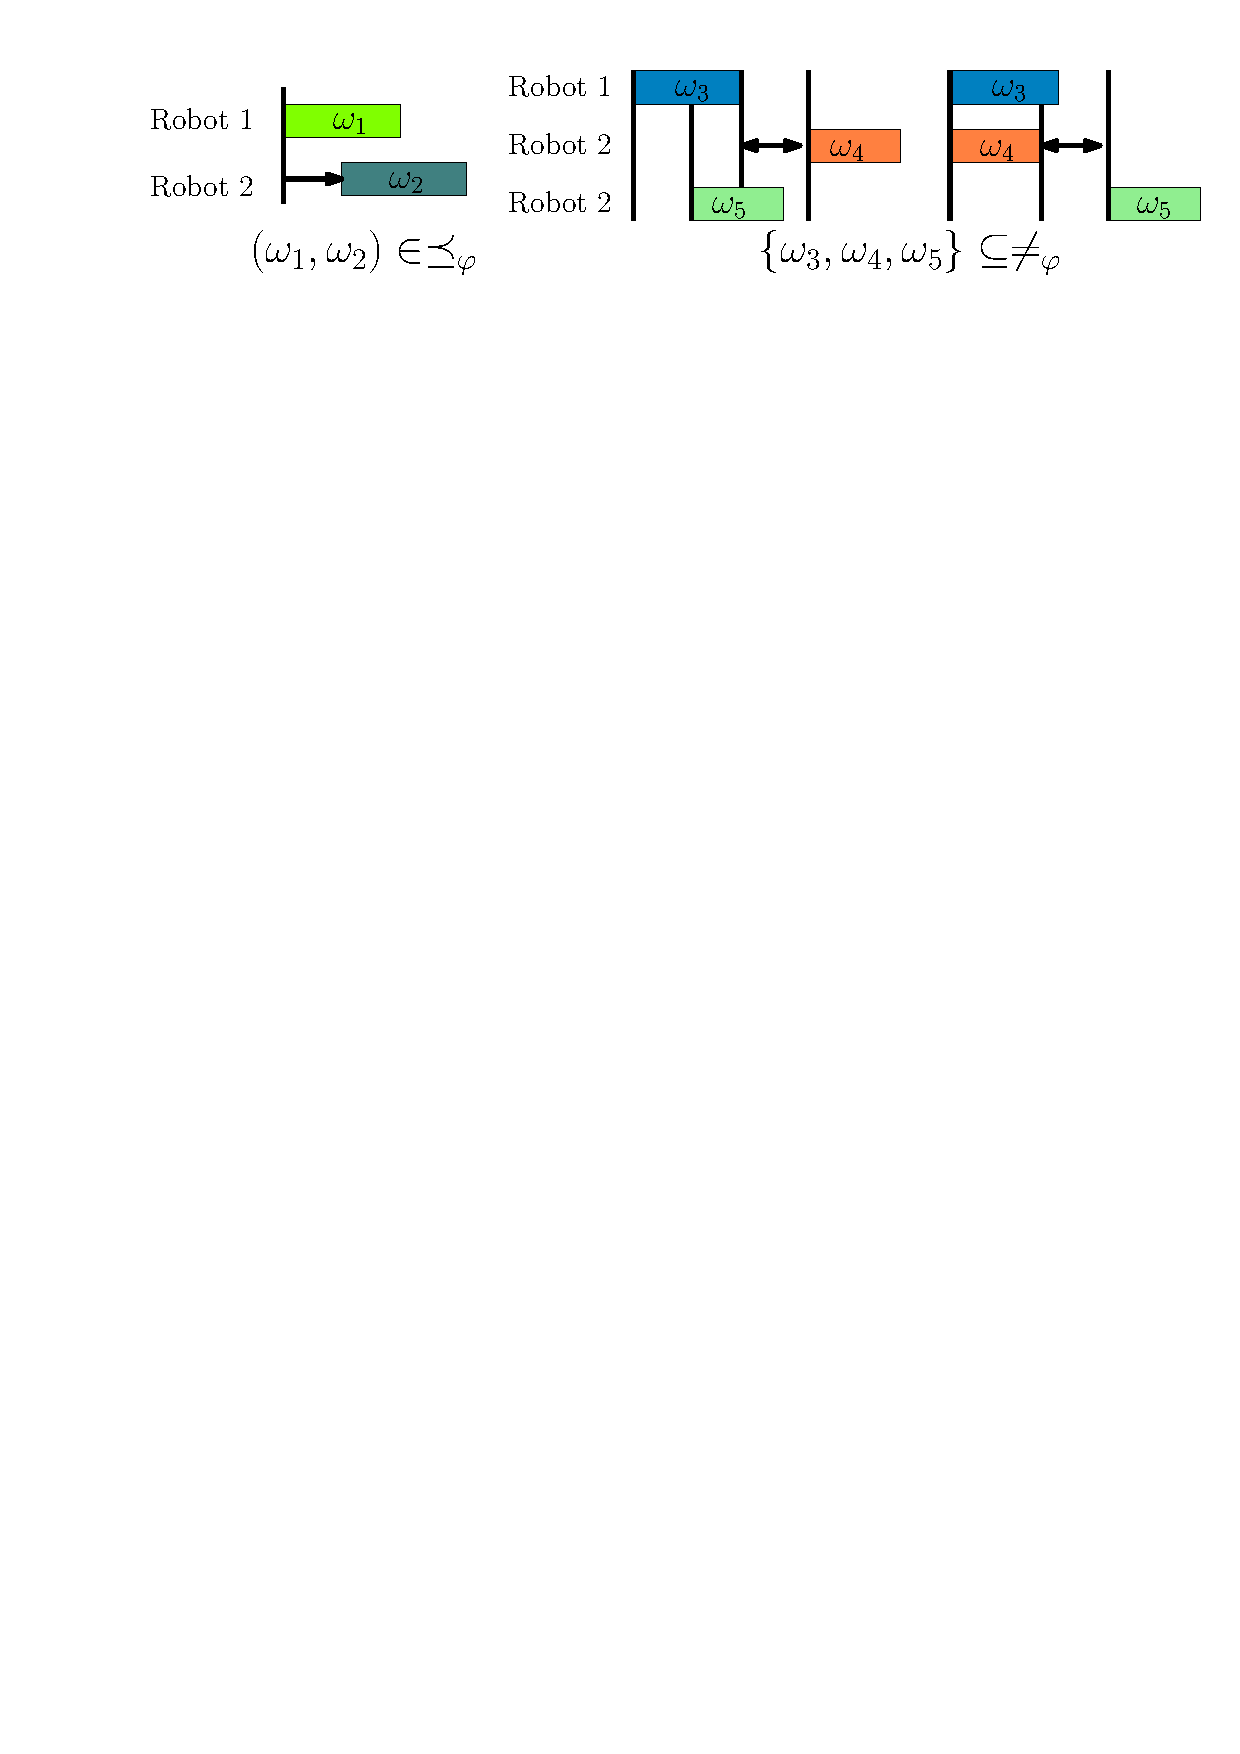
\includegraphics[width=0.95\linewidth]{figures/poset_graph2.pdf}
\centering
%--------------------
\caption{Illustration of the two partial relations
        contained in the poset.
        \textbf{Left}: $\omega_1\preceq_{\varphi} \omega_2$ requires that
task~$\omega_2$ is started after task~$\omega_1$.
\textbf{Middle\&Right}:
$\{\omega_3,\omega_4,\omega_5\}\subset\neq_{\varphi}$
requires that $\omega_3,\omega_4,\omega_5$ are not executing simultaneously.}
\label{fig:partial}
%--------------------
\end{figure}
%========================================

To satisfy a given poset, the language of the underlying system is
much more restricted.
In particular, the language of a poset is defined as follows.

\begin{definition}[Language of Poset]\label{def:language-poset}
Given a poset $P_\varphi=(\Omega_{\varphi}, \, \preceq_{\varphi}, \, \neq_{\varphi})$,
its language is defined as the set of all finite words
that can be generated by the subtasks in~$\Omega_{\varphi}$
while satisfying the partial constraints.
More concretely, the language is given by
$L(P_\varphi)=\{W_{\varphi}\}$, where $W_{\varphi}$ is a finite
\emph{word} constructed with the set of subtasks in $P_\varphi$, i.e.,
\begin{equation}\label{eq:poset-language}
W_{\varphi}=(t_1,\omega_1) (t_2,\omega_2)\cdots (t_L,\omega_L),
\end{equation}
where the subtask~$\omega_\ell \in \Omega_\varphi$ and
$t_\ell$ is the starting time of subtask $\omega_\ell$.
Furthermore, $W_{\varphi}$ should satisfy the partial relations in $P_\varphi$, namely:
(i) $t_\ell \leq t_{\ell'}$ holds,
$\forall (\omega_\ell,\,\omega_{\ell'})\in \preceq_{\varphi}$;
(ii) $\forall \{\omega_{i}\}\subseteq \neq_{\varphi},
\exists\omega_{\ell},\omega_{\ell'}\in\{\omega_{i}\}, t_\ell + d_\ell <  t_{\ell'}$ holds,
where $d_\ell$ and $d_{\ell'}$ are the durations of
subtasks~$\omega_\ell, \omega_{\ell'} \in \Omega_{\varphi}$.
With a slight abuse of notation, $W_\varphi$ can also denote the
simple sequence of alphabets~$\omega_1\omega_2\cdots \omega_L$.
\hfill $\blacksquare$
\end{definition}

Given the above definition, a poset $P_\varphi$ is called \emph{accepting}
if its language satisfies the original task specification, i.e.,
$L(P_\varphi)\subseteq L_\varphi$.
In other words, instead of directly searching for the accepting word of~$\varphi$,
we can focus on finding the accepting poset that
requires the least completion time.
In the rest of this section, we present how this can be achieved efficiently
in real-time.
First of all, it is worth pointing out that it is computationally expensive to
generate the \emph{complete} set of all accepting poset
and then select the optimal one.
More precisely, even to generate \emph{all} accepting runs in $\mathcal{B}_{\varphi}^-$,
the worst-case computational complexity is~$\mathcal{O}(|Q^-|!)$.
Instead, we propose an anytime algorithm that can generate at least one
valid poset within any given time budget,
while adding more posets as time allows.


%==============================
\begin{algorithm}[h]\footnotesize
	\caption{$\texttt{compute\_poset}(\cdot)$: Anytime algorithm to compute accepting posets.}
	\label{alg:compute-poset}
	\SetKwInOut{Input}{Input}
	\SetKwInOut{Output}{Output}
	\Input {Pruned NBA~$\mathcal{B}_{\varphi}^{-}$, time budget $t_0$.}
	\Output{Posets $\mathcal{P}_{\varphi}$, language~$\mathcal{L}_{\varphi}$.}
	Choose initial and final states $q_0\in Q_0^-$ and $q_f\in Q_F^-$;\\
	Set $\mathcal{L}_{\varphi}=\mathcal{P}_{\varphi}=\emptyset$;\\
	Begin modified DFS to find an accepting run $\rho$;\\
	\While{$time<t_0$}{
		\tcc{Subtask decomp. by Def.~\ref{def:subtasks}}
		Compute~ $\Omega$ and word~$W$ given~$\rho$;
		\label{alg-line:decompose}\\
		\If{$W \notin \mathcal{L}_\varphi$\label{alg1:inlp}}{
			Set~$P=(\Omega,\, \preceq_{\varphi}=\mathbb{F},\neq_{\varphi}=2^{\Omega})$,
			and $\preceq_{\varphi}=\mathbb{F}$;\label{alg-line:initial}\\
			Set~$L(P)=Que=\{W\}$ and~$I_1=I_2=\emptyset$;\\
			\tcc{Reduce partial relations}
			\While{$|Que|>0$\label{alg1:begin_que}}{
				$W \leftarrow Que.pop()$;\\
				\For{$i=1,2,\cdots,|W|-1$}{
					$\omega_{1}=W[i]$, $\omega_{2}=W[i+1]$;\\
					$W' \leftarrow $ Switching~$\omega_{1}$
					and~$\omega_{2}$ within~$W$\label{alg1:switch};\\
					\eIf{$W'$ is accepting\label{alg1:waccepting}}{

						Add $(\omega_{1},\,\omega_{2})$ to $I_1$;\\
						Add $W'$ to $Que$ if not in $Que$;\\
						Add $W'$ to $L(P)$ if not in $L(P)$;\label{alg1:add-w}
					}{Add $(\omega_{1},\,\omega_{2})$ to $I_2$;\label{alg1:end_que}}
				}
				Remove $\{I_1\,\backslash\, I_2\}$
				from~$\preceq_{\varphi} $;\label{alg-line:remove}}
				\For{$\{\omega_i\} \subseteq \neq_{\varphi}$\label{alg-line:calculate_neq}}{
				$W' \leftarrow $ Replace~$\omega_i\in\{\omega_i\}$ in~$W$
				by~$\bigcup\omega_i$;\label{alg1:word-neq}\\
				\If{$W'$ is accepting\label{alg1:waccepting-neq}}{
					Remove~$\{\omega_i\}$
					from~$\neq_{\varphi}$;\label{alg-line:remove_neq}\\}
			}
			\tcc{Self-loop calculation }\For{$W$ in $L(P)$}{
				Get path $\rho'$ associated with $\sigma_\ell$ of $W'$;\\
				\For{$i=0,1,\cdots,|\rho'|$\label{alg-line:self-loop}}{
					$\sigma^p_{\ell_1}=\sigma^p_{\ell_1}\cap\delta^{-1}(\rho'[i-1],\, \rho'[i-1])$;\\
			}}
			Add~$P$ to~$\mathcal{P}_{\varphi}$,
			add~$L(P)$ to~$\mathcal{L}_{\varphi}$;}
		Continue the modified DFS, and update~$\rho$;
	}
	\Return{$\mathcal{P}_{\varphi}$,~$\mathcal{L}_{\varphi}$};
\end{algorithm}




As summarized in Alg.~\ref{alg:compute-poset},
the proposed algorithm builds upon the modified depth first search (DFS)
algorithm with local visited sets~\citep{sedgewick2001algorithms}.
Given the pruned automaton~$\mathcal{B}_{\varphi}^-$,
the modified DFS can generate an accepting run $\rho$ given the chosen pair of
initial and final states.
Given $\rho$, the associated set of subtasks $\Omega$ and word $W$ can be
derived by following Definition~\ref{def:subtasks}, see Line~\ref{alg-line:decompose}.
Then, a poset $P$ is initialized as $P=(\Omega,\, \mathbb{F},\, 2^{\Omega})$
in Line~\ref{alg-line:initial},
namely, a fully-ordered poset as described after Definition~\ref{def:poset}.
Furthermore, to reduce the partial relations,
we introduce a ``swapping'' operation to change the order of adjacent alphabets,
and then check if the resulting new word can lead to an accepting run.
If so, it means the relative ordering of this two adjacent subtasks can
potentially be relaxed or removed from~$\preceq_{\varphi}$ as in Line~\ref{alg-line:remove}.
On the contrary, for any other word within~$L(P)$, if such swapping does not
result in an accepting run, it is definitively kept in the partial ordering.
The resulting poset is a new and valid poset that have less partial
ordering constraints.
Furthermore, for any subtasks set that belong to the ``opposed'' relation,
a new word is generated by allowing all subtasks to be fulfilled simultaneously
in Line~\ref{alg1:word-neq}.
If this new word is accepting, it means that this subtasks set do not belong to the
relation~$\neq_{\varphi}$ in Line~\ref{alg-line:remove_neq}. After that, self-loop $\sigma^s_\ell$ is calculated
by checking all feasible word in line~\ref{alg-line:self-loop}.
Note that the resulting~$P$ is only one of the posets and the associated language is
given by~$L(P)$ as defined in~Definition~\ref{def:language-poset}.
Lastly, as time allows, the DFS continues until a new accepting run is found,
which is used to compute new posets with same steps.

\begin{example}
	Continuing from example~\ref{example:subtask}, we can get a poset with
	$\preceq_\varphi=\{(1,2),(1,3)\},\neq_{\varphi}=\{\{2,3\}\}$.
        \hfill $\blacksquare$
\end{example}

%==============================
\begin{lemma}\label{lemma:accepting-poset}
Any poset within $\mathcal{P}_{\varphi}$ obtained by Alg.~\ref{alg:compute-poset}
is accepting.
\end{lemma}
\begin{proof}
Due to the definition of accepting poset, it suffices to show that the
language~$L(P)$ derived above for reach~$P$ is accepting.
To begin with, as shown in Line~\ref{alg1:add-w}, any word~$W$ added to~$L(P)$
is accepting.
Second, assume that there exists a word~$W\in L_\varphi$ but $W\notin L(P)$, i.e.,
$W$ satisfies the partial ordering constraints in~$P$ but does not belong to $L(P)$.
Regarding the ordering relation~$\preceq_{\varphi}$,
due to the iteration process of~$Que$ in Line~\ref{alg1:begin_que}-\ref{alg1:end_que},
any accepting word~$W$ that satisfies the ordering constraints will be added
to~$L(P)$.
In other words, starting from the initial word~$W_0$ associated with the run~$\rho$,
there always exists a sequence of switching operation in Line~\ref{alg1:switch} that results
in the new word~$W$.
With respect to each ordering relation within~$\neq_{\varphi}$, it is even simpler
as any word within~$L(P)$ satisfies this relation and is verified to be accepting
after augmenting the alphabets with the union of all alphabets.
Thus, if~$W\in L_{\varphi}$, it will be first added to~$Que$ in
Line~\ref{alg1:begin_que}-\ref{alg1:end_que} and then
verified in Line~\ref{alg1:word-neq}, thus~$W\in L(P)$. This completes the proof.
\end{proof}



Since Alg.~\ref{alg:compute-poset} is an anytime algorithm,
its output~$\mathcal{P}_{\varphi}$ within the given time budget
could be much smaller than the actual complete set of accepting posets.
Consequently, if a word~$W$ does not satisfy
any poset~$P\in \mathcal{P}_{\varphi}$, i.e.,~$w\notin \mathcal{W}_{\varphi}$,
it can still be accepting.
Nonetheless, it is shown in the sequel for completeness analyses that
given enough time, Alg.~\ref{alg:compute-poset} can generate
the complete set of posets.
In that case, any word that does not satisfy any poset
within~$\mathcal{P}_{\varphi}$ is surely not accepting.
It means that the complete set of posets~$\mathcal{P}_{\varphi}$ is
equally expressive as the original NBA $\mathcal{B}^-$.
The above analysis is summarized in lemma~\ref{lemma:complete-poset}.

%==============================
\begin{lemma}\label{lemma:complete-poset}
The outputs of Alg.~\ref{alg:compute-poset}
satisfy that~$L(P_i)\cap L(P_j)=\emptyset$, $\forall i\neq j$,
and $L(P_i)\subset  \subset L_\varphi$, $\forall P_i \in \mathcal{P}_\varphi$.
Moreover, given enough time~$t_0\rightarrow \infty$,
the complete set of posets can be returned, i.e.,
$L_\varphi = \cup_{P_i\in \mathcal{P}_\varphi}\,L(P_i)=L_\varphi$.
\end{lemma}
\begin{proof}
The first part can be proven by contradiction.
 Assume that there exists two posets~$P_1,\,P_2\in \mathcal{P}_\varphi$
 and one accepting word~$W\in L_\varphi$ such that~$w\in L(P_1) \cap \in L(P_2)$ holds.
Since the set of subtasks within the poset is simply
 the union of all subtasks within each word,
 it implies that~$\Omega_1 = \Omega_2$.
 Then, as discussed in Lemma~\ref{lemma:accepting-poset},~$W\in L(P_1)$ implies
 that there exists a sequence of switching operations that maps the original
 word~$W_0$ to~$W$, all of which satisfy the partial relations in~$P_1$.
 The same applies to~$W\in L(P_2)$.
 Since the set of subtasks are identical, it implies that the relations in~$P_1$
 is a subset of those in~$P_2$, or vice versa.
 However, since the~$Que$ in Alg.~\ref{alg:compute-poset} iterates through all
 accepting words of the same~$\Omega$,
 the partial relations are the maximum given the same~$\Omega$,
 Thus both partial relations in~$P_1, P_2$ can only be equal and~$P_1=P_2$ holds.
Regarding the second part,
the underlying DFS search scheme in Alg.~\ref{alg:compute-poset} is guaranteed
 to exhaustively find all accepting runs of~$\mathcal{B}^-_{\varphi}$.
 Namely, the complete set of posets~$\mathcal{P}_{\varphi}$ returned
 by the algorithm after full termination is ensured to cover all
 accepting words of the NBA.
 As discussed earlier, the pruning procedure does not effect
 the complete set of accepting words.
 Thus, it can be concluded that the returned language set~$L_\varphi$
 is equivalent to the original task specification.
\end{proof}
%==============================

%========================================
\begin{figure}[t!]
	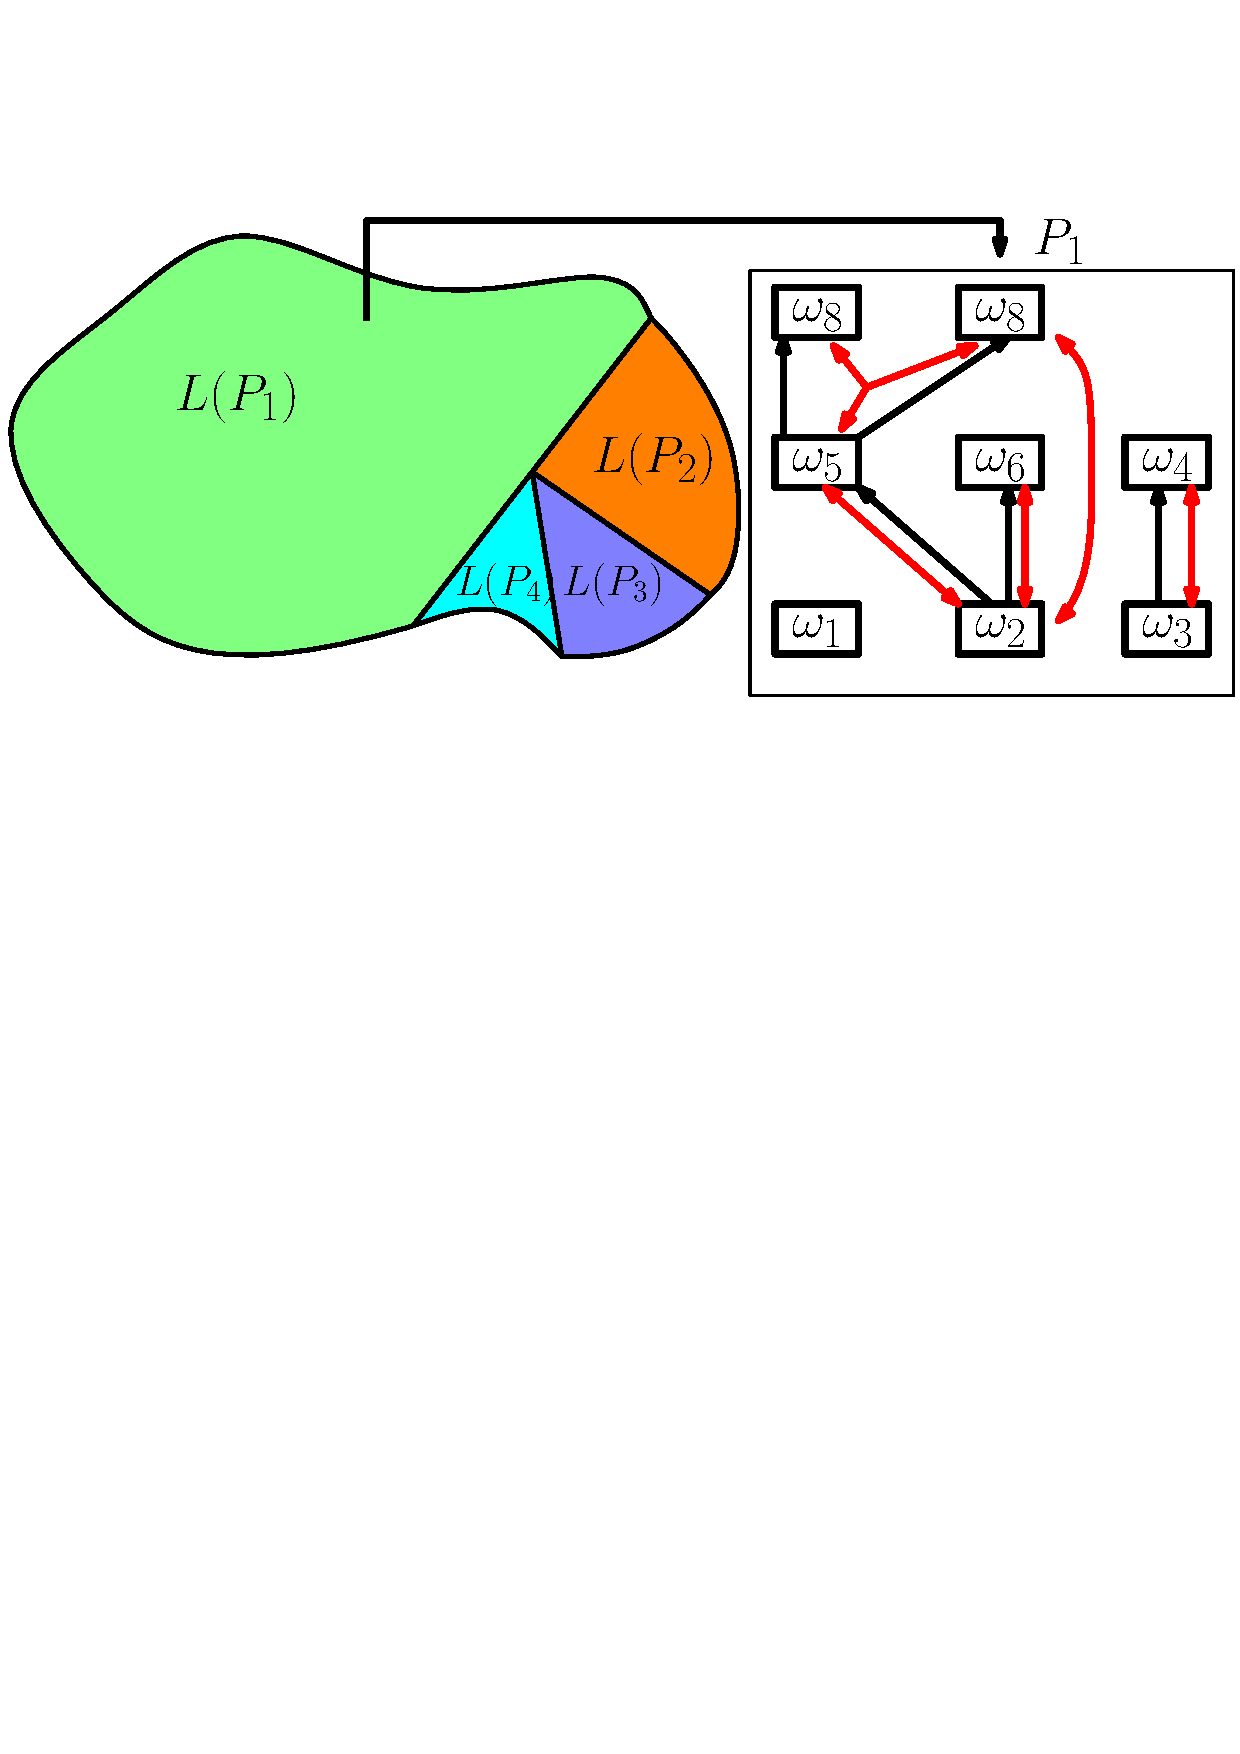
\includegraphics[width=0.85\linewidth]{figures/poset_language2.pdf}
	\centering
	%--------------------
\caption{\textbf{Left}:
an illustration of the relation between the accepting
language of different posets~$L(P_i)$
and the accepting language of the task~$L_\varphi$.
\textbf{Right}:
an example of the poset graph~$\mathcal{G}_{P_\varphi}$,
where the relations~$\preceq_{\varphi}$ and~$\neq_{\varphi}$
are marked by black and red arrows, respectively.}
\label{fig:poset_language}
%--------------------
\end{figure}
%========================================

Similar to the Hasse diagram in~\citep{simovici2008mathematical},
the following graph can be constructed given one poset~$P_{\varphi}$.

\begin{definition}[Poset Graph]\label{def:poset-graph}
The poset graph of $P_{\varphi}=(\Omega,\,\preceq_{\varphi},\,\neq_{\varphi},
\,\Omega_0)$ is a digraph $\mathcal{G}_{P_\varphi}=(\Omega,\,E,\,R)$,
where $\Omega$ is the set of nodes;
$E\subset \Omega \times \Omega$ is the set of directed edges;
$R\subset 2^\Omega$ is the set of undirected special 'edges' which
connect multiple nodes instead of only two.
A edge $(\omega_1,\,\omega_2)\in E$ if two conditions hold:
(i) $(\omega_1,\, \omega_2)\in \preceq_{\varphi}$;
{and} (ii) there are no intermediate nodes~$\omega_3$ such that
$\omega_1\preceq_{\varphi} \omega_3 \preceq_{\varphi} \omega_2$ holds;
lastly, $\Omega_0\subseteq \Omega$ is set of root nodes that do not have
incoming edges. An undirected 'edge' $(\omega_1,\omega_2,\dots)\in R$, if $\{\omega_1,\omega_2,\dots\}\in \neq_{\varphi}$.
\hfill $\blacksquare$
 \end{definition}

The poset graph~$\mathcal{G}_{P_\varphi}$ provides a straightforward
representation of the partial ordering among subtasks,
i.e., from low to high in the direction of edges.
As shown in Fig.~\ref{fig:poset_language},~$\mathcal{G}_{P_\varphi}$ can be dis-connected with multiple root nodes.

%% \begin{example}\label{example:hasse}
%% As shown in Fig.~\ref{fig:poset_language},
%% the associated poset is given by:
%% $\Omega =\{\omega_1,\cdots, \omega_8\}$,
%% $\preceq_\varphi=\{(\omega_2,\omega_5),(\omega_2,\omega_6),(\omega_2,\omega_7),
%% (\omega_2,\omega_8),(\omega_5,\omega_7),(\omega_5,\omega_8)\}$,
%% and $\neq_\varphi=\{(\omega_2,\omega_5),(\omega_2,\omega_6),(\omega_2,\omega_7),
%% (\omega_5,\omega_7),(\omega_5,\omega_8),(\omega_3,\omega_4)\}$.
%% Note that some edges of~$\preceq_{\varphi}$ are omitted due to
%% the transitivity property of~$\preceq_{\varphi}$.
%% For instance, $(\omega_2,\omega_7)$ is removed as it can be inferred
%% by~$(\omega_2,\omega_5),(\omega_5,\omega_7)$.
%% \hfill $\blacksquare$
%% \end{example}
